%Chapter "Wave propagation"
%

\chapter{Wave propagation problems in the time domain}

\section{Problem formulation}

\section{Explicit time integration algorithm}

\section{Statement of the Problem}
Consider the discrete dynamic equilibrium equations at time $t$

\begin{equation}
M^{t}A+C^{t}V+K^{t}U=^{t}F
\label{equil}
\end{equation}

where $M$, $C$, $K$ are the assembled mass, damping and stiffness matrix respectively and similarly $^{t}A$, $^{t}V$, $^{t}U$, $^{t}F$ are the nodal accelerations, velocities, displacements and external loads vectors at time $t$. In terms of forces, \cref{equil} can be written like;

\begin{equation}
^{t}F^I+^{t}F^D+^{t}F^s=^{t}F
\label{force equil}
\end{equation}

where $^{t}F^I$, $^{t}F^D$ and $^{t}F^s$ are inertial, damping and elastic nodal forces respectively.

Expanding the acceleration and velocity terms at time $t$ in a consistent finite central differences scheme we have;

\begin{equation}
\begin{aligned}
^{t}A&=\dfrac{1}{\Delta t^2}\left(^{t-\Delta t}U-2^{t}U+^{t+\Delta t}U\right)\\
^{t}V&=\dfrac{1}{2\Delta t}\left(-^{t-\Delta t}U+^{t+\Delta t}U\right)
\end{aligned}
\label{finitediff}
\end{equation}

It is convenient to write \cref{finitediff} like;

\begin{equation}
\begin{aligned}
{}^tA & = {}^t\hat A + \frac{1}{{\Delta {t^2}}}{}^{t + \Delta t}U\\
{}^tV & = {}^t\hat V + \frac{1}{{2\Delta t}}{}^{t + \Delta t}U
\end{aligned}
\label{precorr}
\end{equation}

where:

\begin{equation}
\begin{aligned}
{}^t\hat A & = \frac{1}{{\Delta {t^2}}}\left( {{}^{t - \Delta t}U - 2{}^tU} \right)\\
{}^t\hat V & =  - \frac{1}{{2\Delta t}}{}^{t - \Delta t}U
\end{aligned}
\label{pred}
\end{equation}

are termed predictors, while $\frac{1}{{\Delta {t^2}}}{}^{t + \Delta t}U$ and $\frac{1}{{2\Delta t}}{}^{t + \Delta t}U$ are termed correctors.

Using \cref{finitediff} in \cref{equil} yields;


\begin{equation}
\left(\dfrac{1}{\Delta t^2}M+\dfrac{1}{2\Delta t}C\right) ^{t+\Delta t}U=^{t}F-M{}^t\hat A - C{}^t\hat V - K{}^tU
\label{resequil}
\end{equation}

or after letting;

\[\hat K = \frac{1}{{\Delta {t^2}}}M + \frac{1}{{2\Delta t}}C\]

and

\[{}^t\hat F = {}^tF - M{}^t\hat A - C{}^t\hat V - K{}^tU\] we have;

\[\hat K{}^{t + \Delta t}U = {}^t\hat P\]

which can be solved for ${}^{t + \Delta t}U$.

\begin{algorithm}[H]
\SetAlgoLined
\KwData{Values at $t=0$, Geometry, Material Paramters}
\KwResult{Displacements, Velocity and Acceleration at any time $t=t$ }
Compute predictors ${}^t\hat A$, ${}^t\hat V$, ${}^t\hat U$\\
Assemble  $\hat K$, ${}^t\hat P$\\
Solve $\hat K{}^{t + \Delta t}U = {}^t\hat P$\\
Perform Corrections ${}^tA \leftarrow {}^t\hat A + \frac{1}{{2\Delta {t^2}}}{}^{t + \Delta t}U$ and ${}^tV \leftarrow {}^t\hat V + \frac{1}{{2\Delta t}}{}^{t + \Delta t}U$
\caption{Explicit algorithm}
\end{algorithm}



%%%%%

Redefine forces as follows
\begin{equation}
\begin{aligned}
^{j}F^I&=\dfrac{1}{\Delta t^2}M ^{j}U\\
^{j}F^D&=\dfrac{1}{2 \Delta t}C ^{j}U\\
^{j}F^S&=K ^{j}U
\end{aligned}
\label{redefine}
\end{equation}

and write \eqref{resequil} as;

\begin{equation}
^{t+\Delta t}F^I+^{t+\Delta t}F^D=^{t}F-^{t}F^s+2 ^{t}F^I-^{t-\Delta t}F^I+^{t-\Delta t}F^D
\label{force equil 2}
\end{equation}

\begin{itemize}
\item \eqref{force equil 2} is an equilibrium equation at time $t=t$ allowing to predict the displacements at time $t=t+\Delta t$ in terms of previously known values at times $t$ and $t=t-\Delta t$.

\item The equation is exact within the error introduced by the expansion used in \eqref{finitediff}.

\begin{figure}[h]
\centering
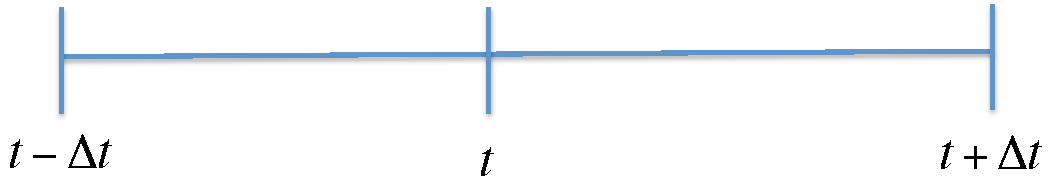
\includegraphics[width=12cm]{img/figure7_0.pdf}
\caption{Definition of the general iteration}
\label{fig:time iteration}
\end{figure}

\item The first predicted solution is at $t=\Delta t$ and we require data at $t=-\Delta t$ and at $t=0$.

\begin{figure}[h]
\centering
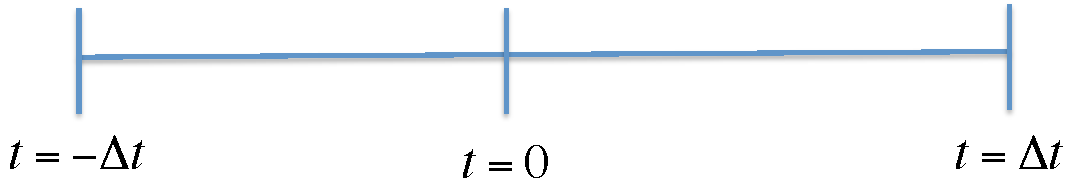
\includegraphics[width=12cm]{img/figure7_1.pdf}
\caption{Definition of the general iteration}
\label{fig:initial time iteration}
\end{figure}

\end{itemize}

\subsection{Damping Assumptions}

\begin{itemize}
\item[1] Use Rayleigh Damping and retain the velocity expansion used in \eqref{finitediff}. That is;

\begin{equation}
C=\alpha M+\beta K
\end{equation}

then we have (in terms of forces);

\begin{equation}
(1+\beta \Delta t^2) ^{t+\Delta t}F^I+\dfrac{\alpha}{2\Delta t} ^{t+\Delta t}F^S=^{t}\hat{F}
\label{Rayleigh}
\end{equation}

where;

\[
^{t}\hat{F}=^{t}R-^{t}F^S+2 ^{t}F^I-^{t-\Delta t}F^I+^{t-\Delta t}F^D
\]

Solution in equation \eqref{Rayleigh} requires the full assembly and factorization of an effective stiffness matrix.

\item[2] Neglect damping (This is however inconvenient for finite domains) 


\begin{equation}
^{t+\Delta t}F^I=^{t}F-^{t}F^S+2 ^{t}F^I-^{t-\Delta t}F^I
\label{Nodamping}
\end{equation}

\item[3] Use Rayleigh damping but modify the velocity expansion introduced in \eqref{finitediff}. Using

\begin{equation}
^{t}V=\dfrac{1}{\Delta t}(^{t}U-^{t-\Delta t}U)
\label{velocity}
\end{equation}

yielding;

\begin{equation}
^{t+\Delta t}F^I=^{t}F-^{t}F^S+2 ^{t}F^{I}-^{t}F^D+^{t-\Delta t}F^D-^{t-\Delta t}F^I
\end{equation}

Defining a set of forces associated to the initial conditions like;

\[
^{t-\Delta t}F^{IC}=^{t-\Delta t}F^I-^{t-\Delta t}F^D
\]

we have

\begin{equation}
^{t+\Delta t}F^I=^{t}F-^{t}F^S+2 ^{t}F^{I}-^{t}F^D-^{t-\Delta t}F^{IC}
\label{modvelocity}
\end{equation}

\end{itemize}

\subsection{Algorithm corresponding to the damping assumption 3}

\begin{figure}[h]
\centering
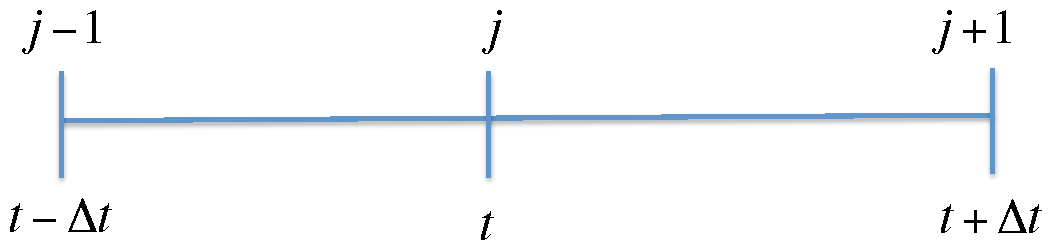
\includegraphics[width=12cm]{img/figure5.pdf}
\caption{Definition of the general iteration}
\label{fig:general iteration}
\end{figure}

Let us write \eqref{modvelocity} like

\begin{equation}
^{j+1}F^I=^{j}F-^{j}F^S+2 ^{j}F^{I}-^{j}F^D-^{j-1}F^{IC}
\label{modveliter}
\end{equation}

where the initialization process corresponds to;


\begin{figure}[h]
\centering
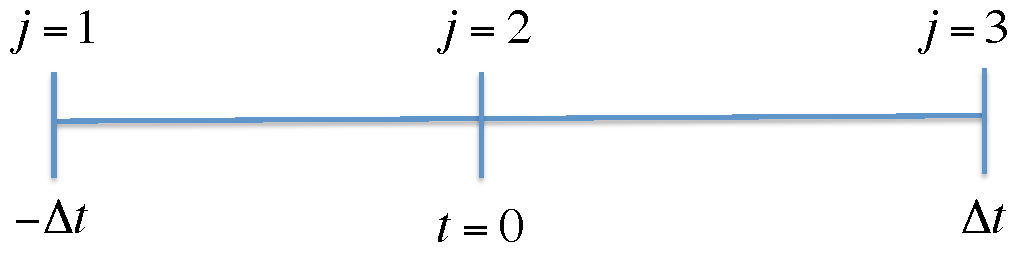
\includegraphics[width=12cm]{img/figure6.pdf}
\caption{Definition of the initial iteration}
\label{fig:initial iteration}
\end{figure}

Applying \eqref{modveliter} for $t=0$ we have;

\[
^{0}F^I=^{0}F-^{0}F^S+2 ^{0}F^{I}-^{0}F^D-^{-\Delta t}F^{IC}
\]

from which it is clear that we require $-^{\Delta t}U$. Applying the central difference expansion at $t=0$ and solving for $-^{\Delta t}U$ yields;

\begin{equation}
^{-\Delta t}U=^{0}F-\Delta t ^{0}V+\dfrac{\Delta t^2}{2} ^{0}A
\label{initialU}
\end{equation}

Using \eqref{initialU} in \eqref{modveliter} allows us to start up the algorithm.

\subsubsection{Particulars}
In what follows we concentrate on this last algorithm and in order to study some details we return to its standard displacements form. Writing \eqref{modveliter} in terms of displacements and re-arranging yields;


\begin{equation}
\dfrac{1}{\Delta t^2}M ^{t+\Delta t}U=^{t}F-(1+\dfrac{\beta}{\Delta t})K ^{t}U+(\dfrac{2}{\Delta t^2}-\dfrac{\alpha}{\Delta t})M ^{t}U-(\dfrac{1}{\Delta t^2} - \dfrac{\alpha}{\Delta t})M ^{t-\Delta t}U+(\dfrac{\beta}{\Delta t}) K ^{t-\Delta t}U
\label{disequil}
\end{equation}

Let;


\[
\begin{aligned}
a_1&=1+\dfrac{\beta}{\Delta t}\\
a_2&=\dfrac{2}{\Delta t^2}-\dfrac{\alpha}{\Delta t}\\
a_3&=\dfrac{1}{\Delta t^2} - \dfrac{\alpha}{\Delta t}\\
a_4&=\dfrac{\beta}{\Delta t}
\end{aligned}
\]


\begin{equation}
^{t+\Delta t}F^I=^{t}F-a_1K ^{t}U+a_2M ^{t}U-a_3M ^{t-\Delta t}U+a_4K ^{t-\Delta t}U
\label{equliassum3}
\end{equation}


\subsection{Decoupling}
Consider the equation for the $i$-th d.o.f;

\begin{equation}
\dfrac{1}{\Delta t^2}M_{ij} ^{t+ \Delta t}U_j=^{t}F_i-a_1K_{ij} ^{t}U_j+a_2M_{ij}^{t}U_j-a_3M_{ij} ^{t-\Delta t}U_j+a_4K_{ij}^{t-\Delta t}U_j
\label{equildecoupled1}
\end{equation}

where we keep $i$ fixed in \eqref{equildecoupled1}. For a lumped mass matrix we can write;

\[
M_{ij}=m_I\delta_{ij}
\]

then \eqref{equildecoupled1} becomes;

\begin{equation}
\dfrac{1}{\Delta t^2}m_I ^{t+ \Delta t}U_i= ^{t}F_I-a_1 K_{ij} ^{t}U_j+a_2 m_I ^{t}U_i-a_3 m_I ^{t-\Delta t} U_i+a_4 K_{ij} ^{t-\Delta t} U_j
\label{equildecoupled2}
\end{equation}

Let;

\begin{equation}
\begin{aligned}
^{t+\Delta t} F_i^I&=\dfrac{1}{\Delta t^2} m_{I} ^{t+\Delta t}U_i\\
^{t} \hat{F}^S_i&=a_1 K_{ij} ^{t}U_j\\
^{t}\hat{F}_i^I&=a_2m_{I} ^{t}U_i\\
^{t-\Delta t}\hat{F}_i^I&=a_3m_{I} ^{t-\Delta t}U_i\\
^{t-\Delta t}\hat{F}_i^S&=a_4K_{ij}^{t-\Delta t}U_j
\end{aligned}
\label{forces2}
\end{equation}

so the recursive equation takes the form;

\begin{equation}
^{t+\Delta t} F_i^I=^{t}F_i-^{t} \hat{F}^S_i+^{t}\hat{F}_i^I-^{t-\Delta t}\hat{F}_i^I+^{t-\Delta t}\hat{F}_i^S
\label{forces3}
\end{equation}

and the algorithm then reduces to;

\begin{algorithm}[H]
\SetAlgoLined
\KwData{Time span, Geometry, Material Paramters}
\KwResult{Displacements, Velocity and Acceleration time histories }
Compute $^{t+\Delta t} F_i^I$\\
Solve for $^{t+\Delta t}U_i=\left(\dfrac{\Delta t^2}{m_I}\right) ^{t+\Delta t}F_{i}^I$\\
Update $^{t}V_i$, $^{t}A_i$
\caption{Summarized Algorithm}
\end{algorithm}

To initialize the algorithm we apply the FD's equations at $t=0$

\[
\dfrac{1}{\Delta t^2}m_I ^{\Delta t}U_i=^{0}F_i-a_1 K_{ij} ^{0}U_j+a_2 m_I ^{0}U_i-a_3 m_I ^{-\Delta t} U_i+a_4 K_{ij} ^{-\Delta t} U_j
\]

where $^{-\Delta t} U_i$ is obtained from \eqref{initialU}

\begin{equation}
^{-\Delta t}U_i=^{0}U_i-\Delta t ^{0}V_i+\dfrac{\Delta t^2}{2} ^{0}A_i
\label{initialU2}
\end{equation}

The initial acceleration is obtained after assuming homogeneous IC's;

\[
m_{I} ^{0}A_i+C_{ij} ^{0}V_j +K_{ij} ^{0}U_j=^{0}F_i
\]

therefore

\[
\begin{aligned}
m_{I} ^{0}A_i=\dfrac{^{0}F_i}{m_I}\\
^{-\Delta t} U_i=\dfrac{\Delta t^2}{2m_I}^{0}F_i
\end{aligned}
\]

Moreover, neglecting the damping effects on the prediction of $^{\Delta t}U_i$ yields;

\[
^{\Delta t} U_i=\dfrac{\Delta t^2}{2m_I}^{0}F_i
\]

\begin{algorithm}[H]
 \SetAlgoLined
 \KwData{Time span, Geometry, Material Paramters}
 \KwResult{Displacements, Velocity and Acceleration time histories }
 Initialize solution vectors ($j=1$)\;
 $^{0}U_i\longrightarrow ^{1}U_i=0$, $^{0}V_i=0$, $^{1}A_i=\dfrac{^{1}R_i}{m_I}$ \;
 Select $\Delta t$ and integration constants $a_1$,$a_2$, $a_3$, $a_4$\;
 Fix 1-st predicted value (let $j=2$)\;
 \[
^{\Delta t} U_i \longleftarrow \dfrac{\Delta t^2}{2m_I} ^{0}F_i\longleftrightarrow \left[^{2}U_i \longleftarrow\dfrac{\Delta t^2}{2m_I} ^{1}F_i \right]
 \]
Time Integration Phase\;
\While{$j \leq N$}{
\[
\begin{aligned}
^{j+1}F^I_i\longleftarrow& ^{j}F_i-a_1 K_{ij} ^{j}U_j+a_2 m_I ^{j}U_j-a_3 m_I ^{j-1} U_i+a_4 K_{ij} ^{j-1} U_j\\
 ^{j+1}U_i\longleftarrow&\dfrac{\Delta t^2}{2m_I} ^{0}F^I_i\\
 ^{j}A_i\longleftarrow&\dfrac{1}{\Delta t^2}\left(^{j-1}U_i-2^{j}U_i+^{j+1}U_i\right)\\
 ^{j}V_i\longleftarrow&\dfrac{1}{2\Delta t}\left(-^{j-1}U_i+^{j+1}U_i\right)\\
 j\longleftarrow&j+1
\end{aligned}
\]
}
\caption{Full Algorithm}
\end{algorithm}

\subsubsection{Nodal Assembler}
In the uncoupled explicit finite element formulation the equation solving process proceeds one degree of freedom at a time. This implies a different assembly process to the one used in an implicit algorithm where a formal coefficient matrix is assembled and inverted. Now the mass, damping and stiffness elemental matrices are used to obtain effective nodal forces at each degree of freedom. In summary the mesh is not covered in an element by element basis, but in a node by node basis. In the following algorithm we discuss this nodal assembly process where in order to solve the displacement at a given degree of freedom prior knowledge of the element contributing to the given node is necessary. In the nodal assembler algorithm the following arrays are needed.

\noindent
ILIST(): Stores the elements connected to the current node.\\
LPLIST():Stores the local position of the current node in each one of the elements of ILIST().\\
NIEL():Number of elements at the current node. This array is used to access ILIST().\\


\begin{algorithm}[H]
\SetAlgoLined
\KwData{Number of nodal points, number of elements, Model}
\KwResult{Displacements, Velocity and Acceleration time histories }
\While {$i \leq NUMNP$}
{
$K\leftarrow NIEL(i)$
%\while {$ik \leq 2$}{
%$jK \leftarrow ID(ik,i)$
%}
}
\caption{Nodal Assembler}
\end{algorithm}
\section{The DRM approach}





